\documentclass[10pt]{IEEEtran}

\usepackage[hyphens]{url}
\usepackage[pdftex,bookmarksnumbered,hidelinks,breaklinks]{hyperref}
\usepackage{amssymb}
\usepackage{amsmath}
\usepackage{caption}
\usepackage{amsrefs}
\usepackage{courier}
\usepackage{graphicx}
\usepackage{bookman}
\usepackage{amsthm}
\usepackage{verbatim}
\usepackage{xcolor}
\usepackage{setspace}
\usepackage{float}
\usepackage{url}
\usepackage{listings}
%\usepackage{appendix}
\usepackage[margin=1in]{geometry}
\bibliographystyle{amsmath}
\newtheorem{definition}{Definition}
\newtheorem{theorem}{Theorem}
\newcommand{\?}{\stackrel{?}{=}}
\begin{document}

\title{Right Whale Recognition and Classification}
\date{}
\author{Tyler Allen}
\maketitle

%\doublespacing

\begin{abstract}
With less than $500$ North Atlantic Right Whales remaining on earth, scientists
track their health through aerial photographs. This is time consuming, and 
can possibly be improved by machine learning. In this paper we will discuss
using the results of photo recognition as input to neural networks,
and the effectiveness of this method. 
\end{abstract}

\section{Introduction}
North Atlantic Right Whales are an endangered species. Less than $500$ Right
Whales remain\cite{kaggle_desc}. Scientists keep track of the health conditions of the remaining
Right Whales in order to help preserve the species. This process is done by
examining aerial photographs of these whales. Each whale has an identification
number\cite{kaggle_desc}. Identifying these whales is extremely time consuming.
It may be possible to improve this process by introducing machine learning. 
Since photographs are the only source of information, there are two problems
that must be solved to complete this project. First, the whale must be recognized
in the photograph. Second, the whale must be classified with its idenficiation
number. This creates a very complex problem, as it requires the results of 
one machine learning process to be used as input to other machine learning
algorithm. In this paper, we will discuss the approach fo using the \textit{MATLAB}
suite of image recognition tools to do photo recognition, the approach of using
a neural network to classify recognized whales, and the approach of using a 
deep belief network to classify recognized whales. We will see that the approach
of photo recognition presents its own set of issues as input to classification
issues, and discuss the results of using this method. We will also discuss the
lessons learned from this approach, and present potential future work that
could provide better results.
This project is based on a contest by \textit{kaggle.com}\cite{kaggle_desc}. 

\section{Methodology}
\subsection{Data}
The data provided for this competition is a set of $11469$ images of Right 
Whales collected over the course of ten years\cite{kaggle_data}. These 
images vary by angle and resolution, and they may contain a number of attributes 
considered to be
noise. This can be seen by contrasting figures \ref{whale} and \ref{whale2}. 
This noise includes lighting variation, surface reflectivity, surface
disturbance, other whales, dolphins, seagulls, and particles in the water.
Common information such as creation dates and geo tags were removed from the 
photographs prior to distribution. 

\begin{figure}[H]
\begin{center}
\captionsetup{justification=centering}
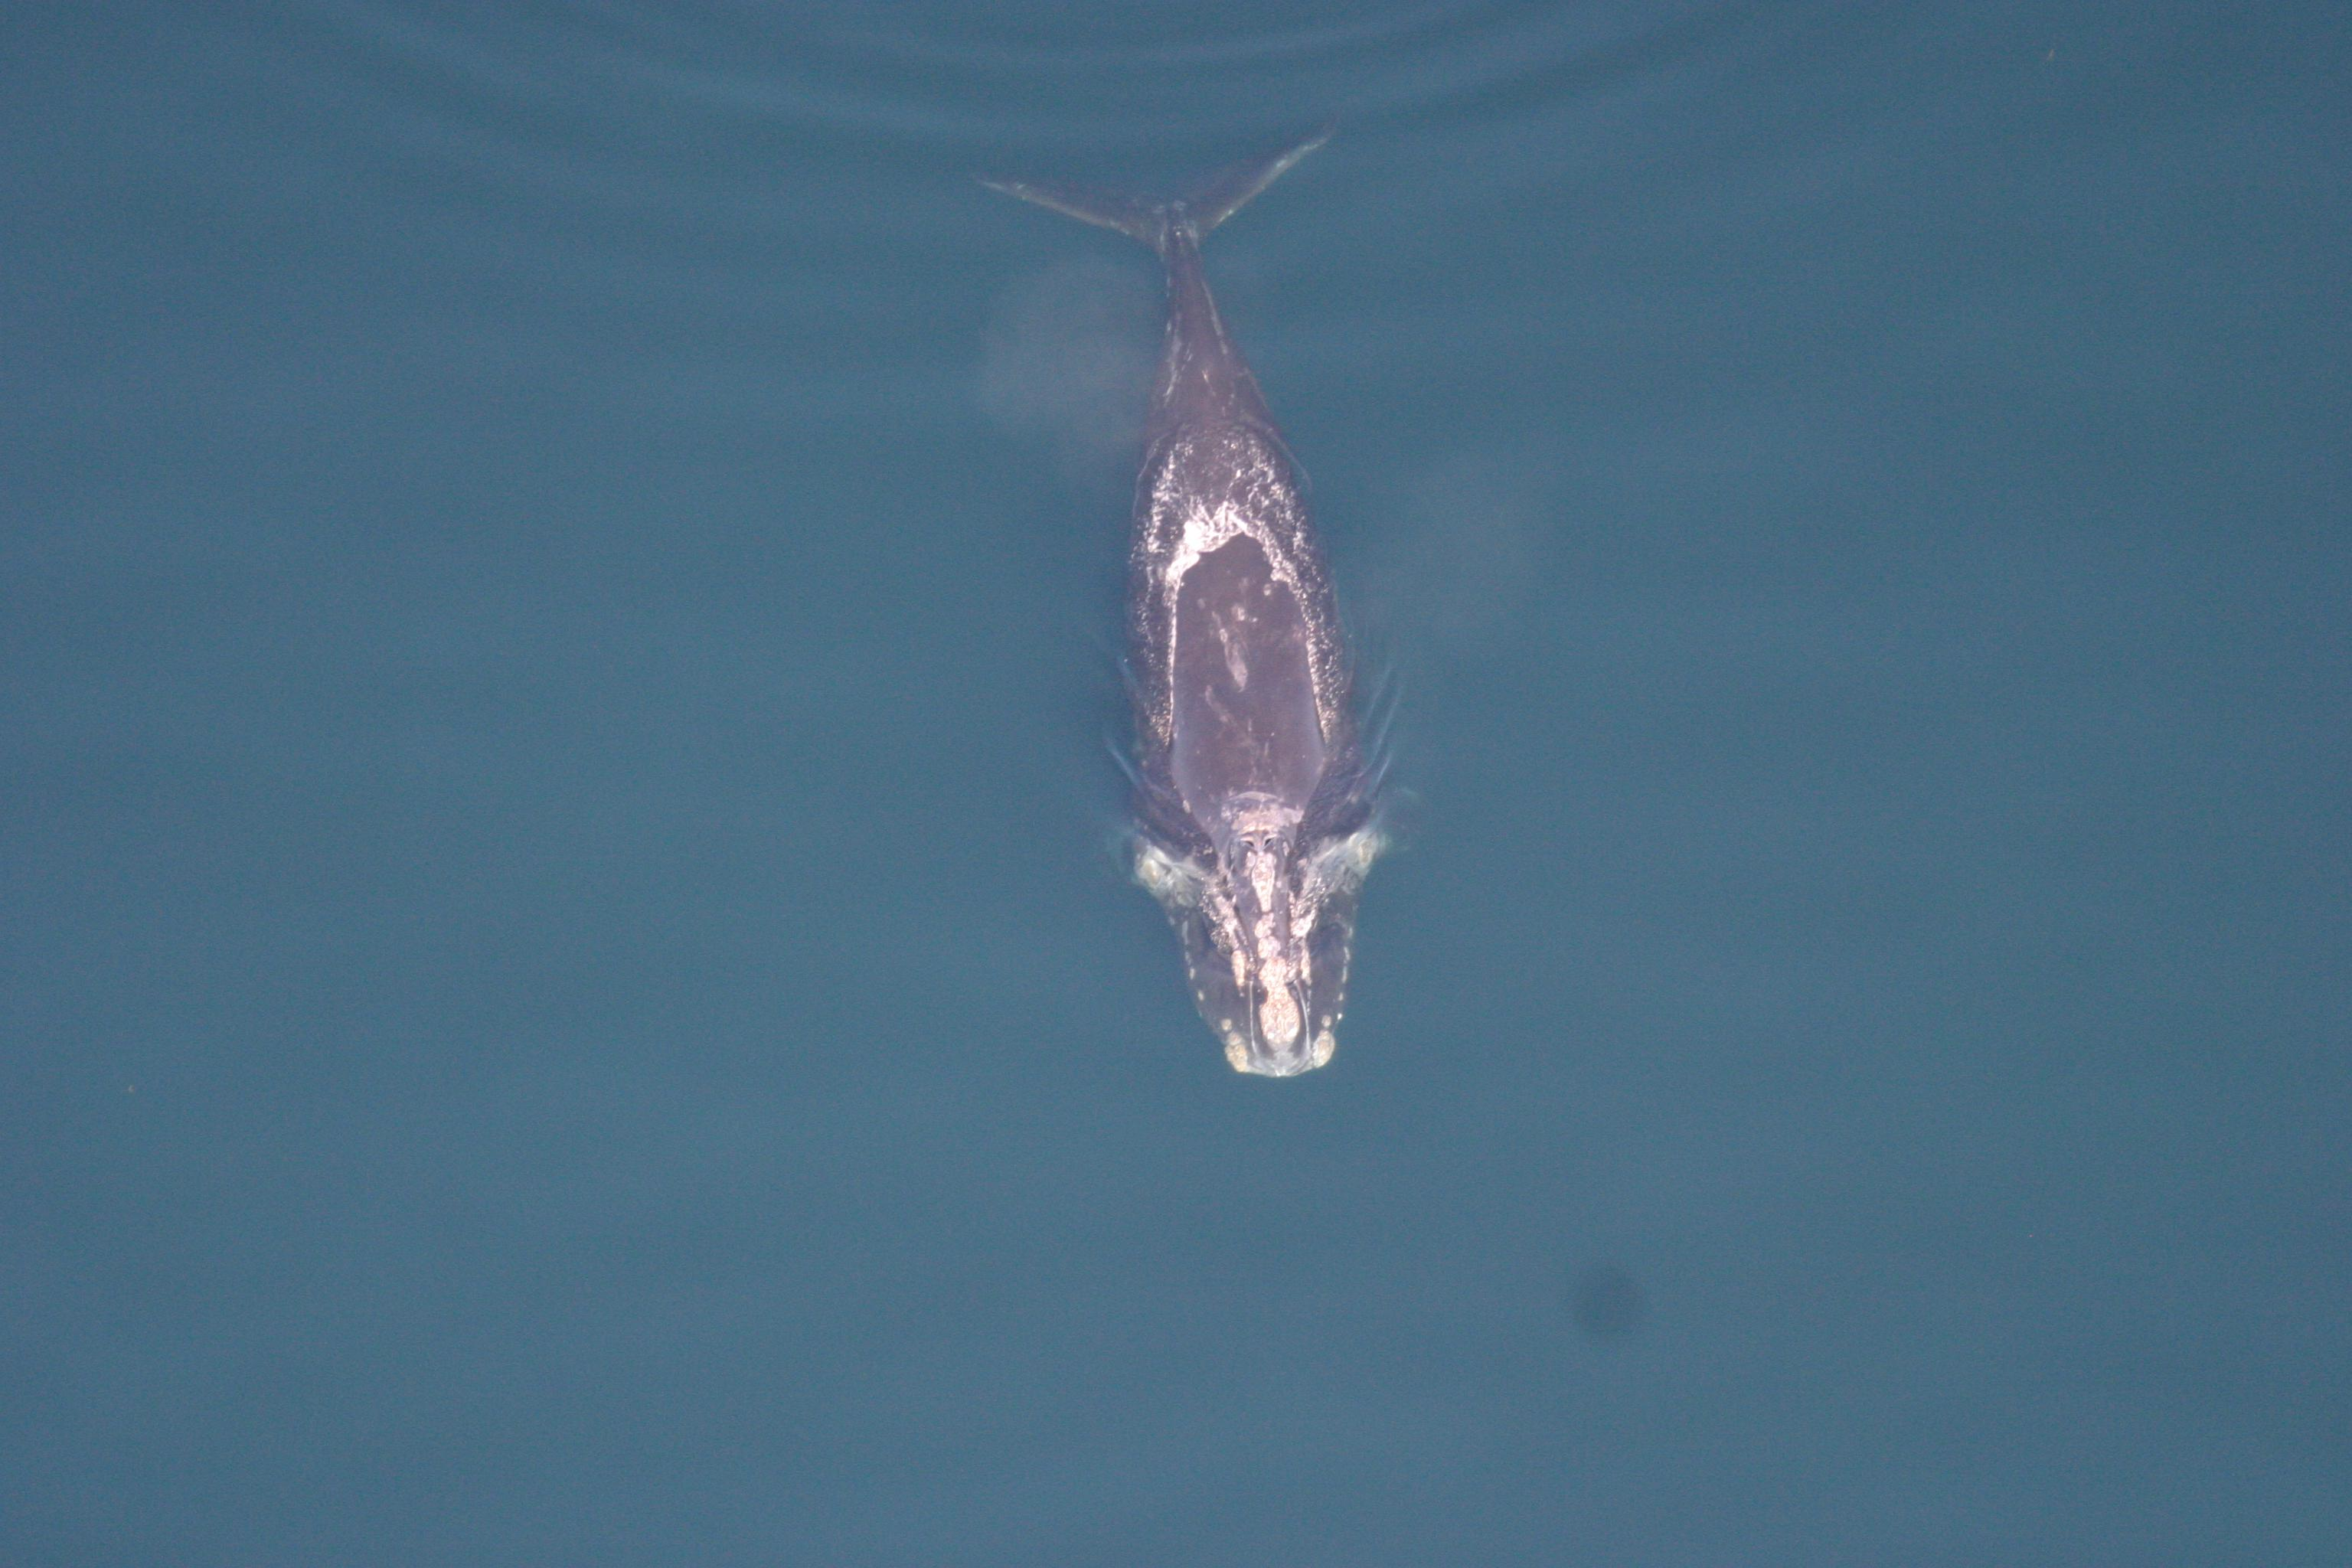
\includegraphics[scale=.06]{whale.png}
\caption{Sample whale photograph.}
\label{whale}
\end{center}
\end{figure}

\begin{figure}[H]
\begin{center}
\captionsetup{justification=centering}
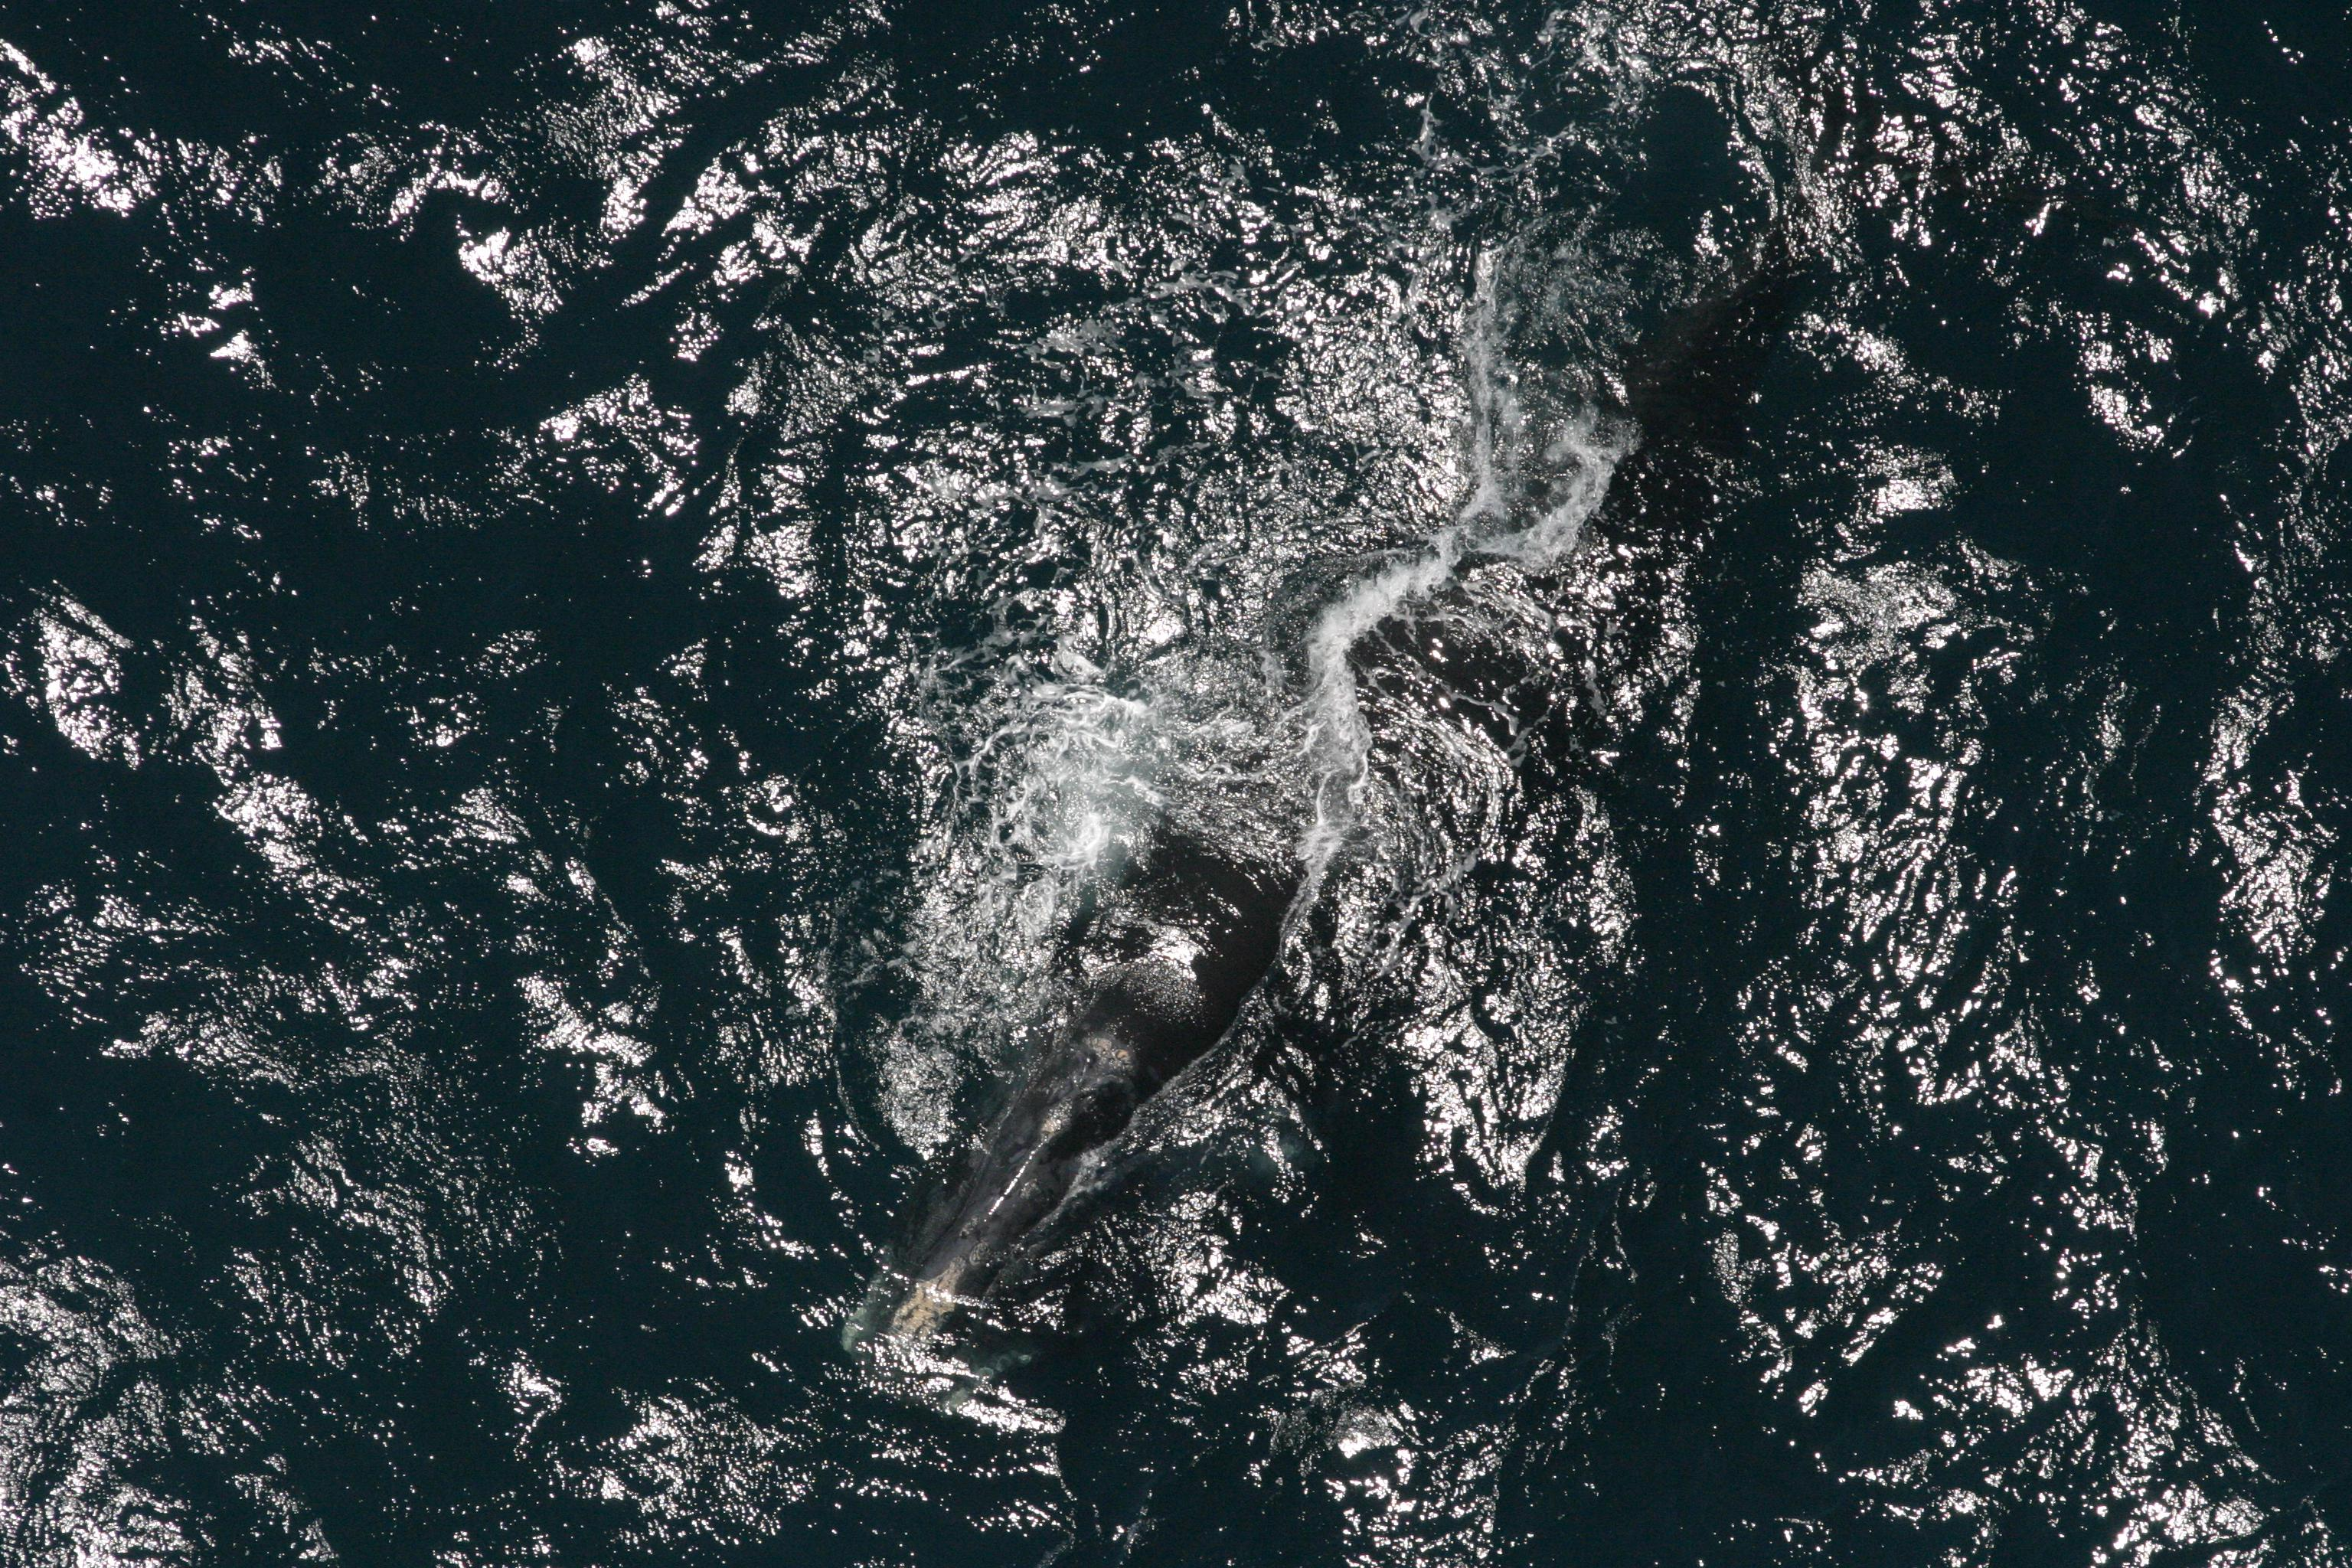
\includegraphics[scale=.06]{whale2.png}
\caption{Whale photos can have a large degree of variation.}
\label{whale2}
\end{center}
\end{figure} 

The training data consists of $4544$ of the original $11469$ images. A list is 
provided containing the file name of each training image along with the 
correct identification number. The contest instructions claim that the
remaining $6925$ images may be ``resized, cropped, or flipped'' to discourage
hand labeling of test data\cite{kaggle_data}. 
~
\subsection{Detection}
Detection was performed by using the \textit{MATLAB} Cascade Object Detector 
software provided as part of the competition\cite{kaggle_face}\cite{math_cascade}. 
This software is a machine learning tool that can be trained to detect objects,
and can be used for tasks such as facial recognition. We chose to use it as 
a ``whale facial recognition'' tool, as was suggested by the contest 
providers\cite{kaggle_face}. Using the full body was considered, but it was 
noted that the photographs frequently did not contain the full body. In addition,
most of the whales seemed to have identifying features (markings) on their faces
that would be ideal features for classification. Due to the previously mentioned
noise in the photographs, no environmental features could be used to identify
the whales.

The cascade object detector requires training input that has been labeled with
a bounding box around the object to be identified. The $4544$ training examples
were hand labeled using the \textit{MATLAB} Training Image Labeler tool. 
This tool allows the user to draw a bounding box an image, and then export the
data for use in later matlab analysis as seen in figure \ref{box}.

\begin{figure}[H]
\begin{center}
\captionsetup{justification=centering}
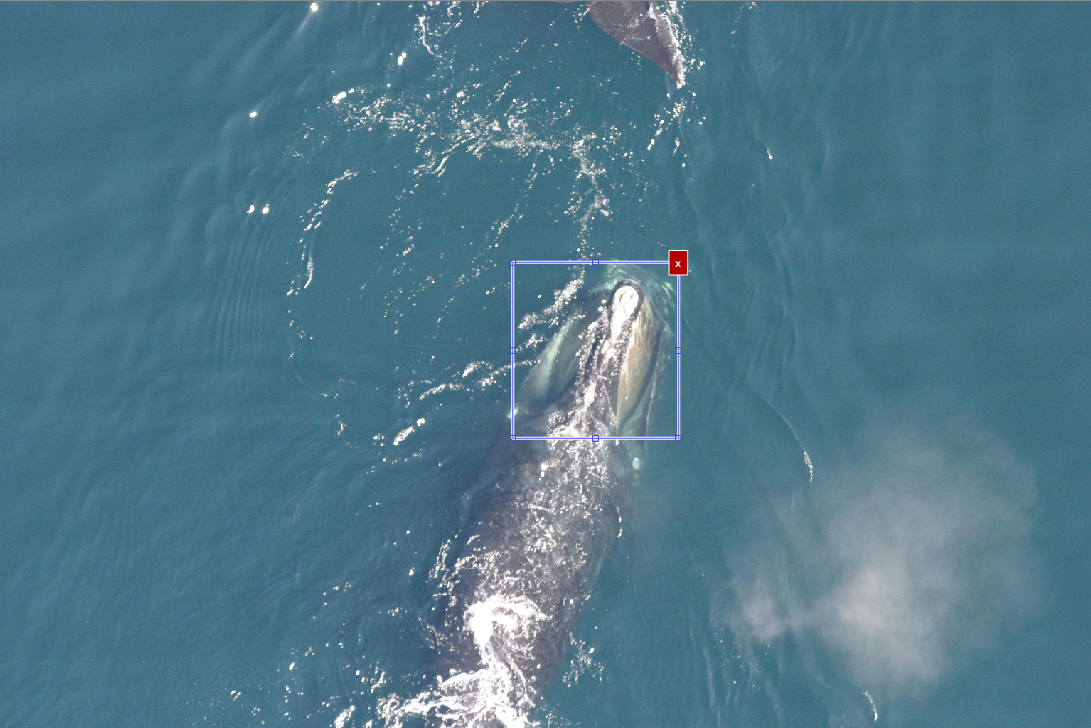
\includegraphics[scale=.2]{box.png}
\caption{A labeled training sample.}
\label{box}
\end{center}
\end{figure} 

The required training parameters to the cascade object detector are 
\texttt{outputXMLFilename}, \texttt{positiveInstances}, 
and \texttt{negativeImages}\cite{cod}.
The parameter \texttt{outputXMLFilename} is simply the location to store data.
\texttt{positiveInstances} is the exported data from the Training Image Labeler
tool. \texttt{negativeImages} is a directory of negative images. The Cascade
Object Detector requires a number of images not containing whales to help
distinguish between the whales present in the photo and the background noise\cite{cod}.
These photos were procedurally generated by cropping parts of photos where 
whales had already been identified.
Two optional parameters are the \texttt{FalseAlarmRate} and \texttt{NumCascadeStages}.
The false alarm rate is ``the fraction of negative training samples incorrectly
classified as positive samples'', and the number of cascade stages are the number
of times detector should iterate over the training data. The suggested values
were $15$ stages, with a false alarm rate of $0.01$. Experimentation led to 
the use of $7$ stages, and $0.005$ for the false alarm rate. Stages $9$ and 
above generated a program warning indicating that it would not be able to 
sufficiently identify images. Reducing the stages and decreasing the false 
alarm rate seemed to provide more accurate results.


\subsection{Classification}
Classifying large images that have not been normalized is a very challenging
problem. Out of the $4544$ training examples provided, there are $447$ unique
whale identification numbers. Each whale identification number has a varying
number of correlated training examples. One of the $447$ only has a single
associated training image. The appropriate classification methods for this 
type of data must have the ability to understand image input. The correct
methods must also be able to handle noise, because noise is present in the 
iamges. Additional noise is also generated by the Cascade Object Detector 
output, since the correct whale image may sometimes not be chosen. The two
methods chosen were a neural network, and a deep belief network. 

The input to the machine learning programs is the output of the image recognition
stage. To provide a good input format for the neural network, the data was 
normalized. First, the bounding boxes detected by the image recognition stage
were cropped out of their original image. These images were resized to $32x30$
resolution. This value was pulled from a ``face pose'' study of humans contained
in the Machine Learning textbook by Mitchell\cite{mitchell}. This resolution 
is low, but still maintains the features to some extent. Larger images require
more processing time, so this size was chosen to preserve features while reducing
processing time. Figure \ref{resized} is an example of one of these resized 
images. In addition, the photos were converted to greyscale for the neural
network, to reduce the amount of image data by a third, while preserving the 
contrast between whales and their facial markings.

\begin{figure}[H]
\begin{center}
\captionsetup{justification=centering}
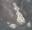
\includegraphics[scale=1]{resized.png}
\caption{Resized sample image at true resolution.}
\label{resized}
\end{center}
\end{figure} 

The neural network was implemented in the Java programming language. It is a 
three layer feedforward neural network using backpropogation for training, as
described in Mitchell\cite{mitchell}. The input layer consists of $960$ input
nodes, which is the product of the $32x30$ resolution. Each input is a single,
in-order, greyscale pixel. The output layer is $447$, one node for each possible whale
identification number classification. The hidden layer is $704$, the average
of the two values. This is due to it being the average of the input output 
layers. This may not be optimal, but training times did not allow for 
validation of this value. The neural network also offered functionality to 
store the state of the network, so that the training results could be reused. 
The learning rate was $0.1$, and the weights began as values between $-0.5$ 
and $.5$, as referenced from Mitchell\cite{mitchell}. The node activation function
was the standard sigmoid function\cite{mitchell}. Each greyscale input was resized
from the range of $0-255$ to a floating point value between $-1$ and $1$.\\
The neural network was written in three iterations. The initial version used
online learning. Due to the extreme runtime required by this version, it was
converted to batch learning as an intermediate step, and then rewritten to make
use of MPI. This would allow training to be done in parallel on the palmetto
cluster in hopes of reducing training time. The MPI version divide the training
images in each epoch to other nodes. Since batch learning was used, each 
image simply had to return its results to be summed by the master. The training 
section of the MPI code is available in appendix \ref{appendix:mpi}.

The deep belief network was implemented using the \textit{Deep Learning 4 Java} (DL4J)
library\cite{dl4j}. The configuration of this network is very similar to the 
previous neural network. It again consists three layers with $960$ input nodes,
 $704$ hidden layer nodes, and $447$ output nodes. A learning rate of $.0000001$
 was used, as suggested by the Deep Belief Network reference page\cite{dbn}. 
 As is consistent with the definition of a Deep Belief Network, the layers
 are constructed of Restricted Boltzmann machines\cite{dbn}. The activation function is a
 rectified linear unit function, again recommended by the Deep Belief Network
 construction page\cite{dbn}. Deep Learning 4 Java provides several techniques
 for parallelization, including multithreading\cite{scaleout}. This allows training to be 
quite a bit faster than the custom neural network. Appendix \ref{appendix:dbn} provides the
code used in the network setup. 


\section{Results}
\begin{figure}[H]
\begin{center}
\captionsetup{justification=centering}
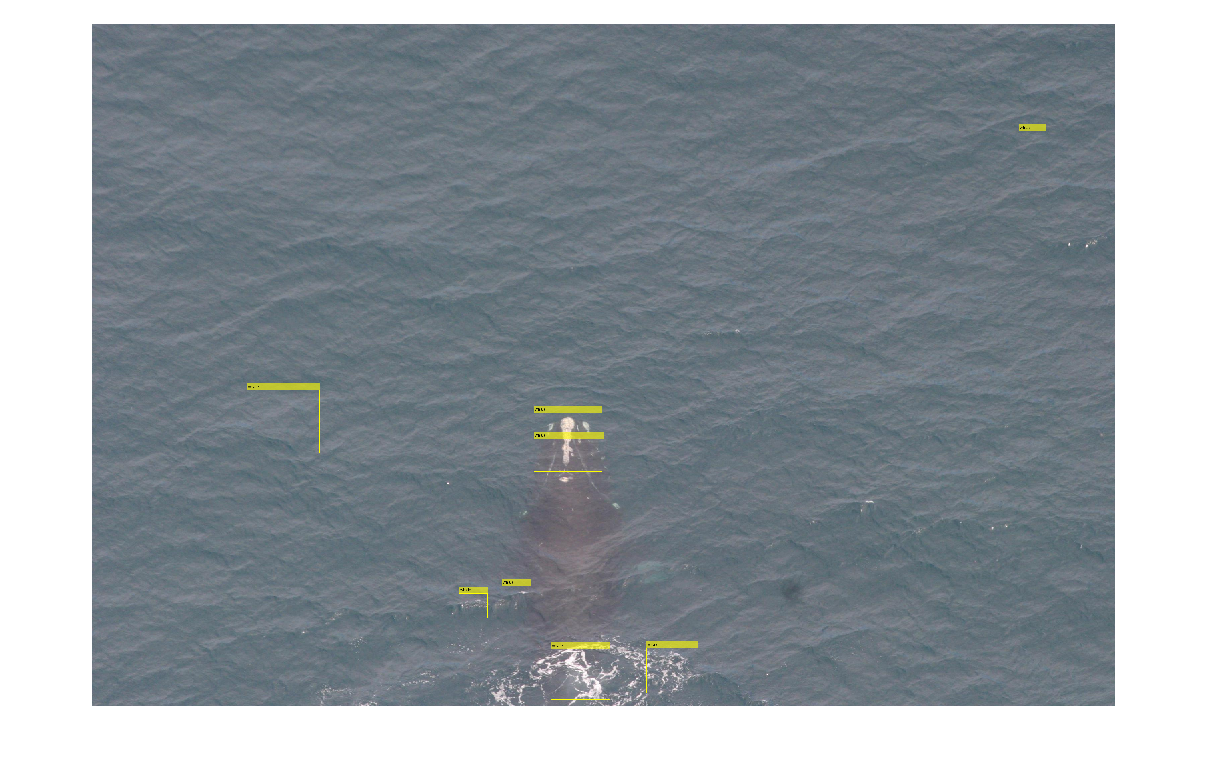
\includegraphics[scale=.25]{detect.png}
\caption{Objects detected by the CascadeObjectDetector.}
\label{detect}
\end{center}
\end{figure} 

The final results of the recognition stage vary quite a bit from image to image.
Ideally, only one bounding box would appear per image. Unfortunately, there
are typically more than one objects detected. Figure \ref{detect} is one example.
The face was accurately detected, but there are several incorrect detections as 
well. Detecting the correct whale out of the selections made is another challenging
task, as adjusting the parameters only seemed to provide minor improvements. No
adjustments prevented most pictures from having false positives.
Unfortunately, we must chose a single one of the detected bounding boxes to 
use for classification. The current implementation chooses a random box of the
ones found. Other methods were investigated, such as searching for the ``most
gray'' bounding box, but the lighting conditions and reflectivity found in 
various images cause this method to skew the data towards certain image qualities.

Results for classification are evaluated using a multi-class logarthmic loss 
method\cite{kaggle_eval}. The perfect result set would have a score of $0$, 
and higher values indicate less correctness. The highest score is currently
$3.02633$, as of December $5^{th}$. 

The basic neural network using batch learning scored a result of $34.49601$ 
on the leaderboard. The neural network was only trained through $100$ iterations. 
This is because training had to restart several times throughout the course of 
this project, and it requires roughly $26$ minutes to do one epoch over the $4544$
training data samples. This means that $100$ iterations required nearly $2$ 
consecutive days. It was not possible to run the simulation continuously for 
several days, so it had to be trained in parts over time. It would have required
 roughly $18$ consecutive days to complete $1000$ iterations. Mitchell succeeded in classifying
 human face position in only $100$ iterations, but the network was much smaller,
 had only $260$ training samples, and had only $4$ possible 
 classifications\cite{mitchell}. Training time is probably not the only issue, as 
 the input from the facial recognition has already been shown to be inaccurate. 
 When input from facial recognition is a false positive, it's possible that the
 neural network partially learns features outside of expectation, such as water
 color.

 The MPI version of the neural network was unable to produce results. When launched
 on palmetto, every node died when the Java Virtual Machine (JVM) failed to initialize
 due to lack of memory. This occurred with both the preinstalled versions of 
 Java and MPI, as well as the versions installed locally to the user account.
 This persisted despite passing arguments to the Java Virtual Machine to 
 allocate more memory on startup. Requesting up to $12$GB of memory per node
 was also insufficient, despite the non-MPI version requiring far less than $12$GB.
 Since the JVM crashed on initialization, the neural network code was never able
 to initialize, so it is most likely a configuration issue with Palmetto. There
 was insufficient time to contact CCIT to resolve this issue in time to provide
 results in this paper. 

The deep belief network had similar issues to the neural network. With $500$
epochs, using $80\%$ of the data as training data, and the remaining $20\%$ as
test data, it received an accuracy score of $.001$, precision of $0.0217$, recall
of $.0909$, and F1 score of $0.0351$. These scores are far below expectation
for a sophisticate neural network. The number of epochs is not recommended directly
for problems like this by Deep Learning 4 Java, but in at least one case $500$
iterations are used\cite{suggestion}. 
\section{Discussion}
\subsection{Lessons Learned}
Machine Learning using images is a challenging problem. Using the output of 
a machine learning algorithm as input to other machine learning algorithms should
not have been my first goal with machine learning. It has been a very interesting
problem to work on, but some prior experience would have prevented a lot of 
difficulty and issues, and likely provided much better results over the course 
of this project.

The \textit{Matlab} Cascade Object Detector may not have been the optimal
tool for facial recognition. An alternative tool, \texttt{haarcascade} from the 
\textit{OpenCV} library was also considered as a replacement for the Cascade 
Object Detector\cite{haar}. This tool was suggested by some users on the Kaggle 
website because in some cases it performed better than the appropriate matlab 
tool\cite{kforums}. This was ruled out, because the classification process 
would be too time consuming to run on two different data sets for comparison.

The neural network was written in Java with the intention of allowing different 
machine learning methods to be designed in an object-oriented fashion so that 
they could be modularly exchanged within the same program. This would have 
provided a good design for analysis and comparison.
In hindsight, the language of implementation probably should have been C or 
C++ to facilitate faster runtimes. However, it is abundantly clear that libraries
such as DL4J provide far greater performance than custom software for
challenging these problems in the real world\cite{scaleout}.

The Deep Learning 4 Java library, while powerful, is very poorly documented. 
The website contains several examples, but none that fit my specific needs.
The associated API documentation is largely absent. It
seemed to be the only common deep learning library available for Java. Java
was chosen for compatability with some of the existing code from the neural network.
This is another area where perhaps C, C++, or other languages may be better 
due to better support.

\subsection{Future Work}
The first step in continuing this project would have to be sorting out the 
issues in the initial photo recognition stage. One possibility would be using
the alternative photo recognizer from \textit{OpenCV}\cite{haar}.
Using the current deep belief network on larger 
scale images, or images that have not been cropped, may be a worthwhile experiment.
In some cases, it is recommended by the Deep Learning 4 Java library not to 
normalize the data\cite{face}. Removing all layers of normalization, and then
adding them back one-by-one, may give an indication of what the
deep belief network expects. Improving the photo recognition stage or finding
a way to collapse the two steps into one step is definitely the 
first goal to continue this project.

There may also be more appropriate methods for use on this project. In late 
November, a post appeared on the contest forums with information about 
Convolution autoencoders\cite{autoencode}. This information was written and 
provided by the person ranked $2^{nd}$ in the Right Whale competition with
the intention to ``level the playing field.'' This seems like a strong direction
to take this project. Another student presented work on the MNIST data set 
using this method as well, and had the best results with it. 

\section{Conclusion}
The main products of this project were a trained whale face recognizer, a neural
network written in Java, and a deep belief network using the Deep Learning 4 Java
library. In general, the resulting accuracy of these scores was very low. It
is believed that this is largely caused by false positives generated 
by the recognition step. Since these results were fed into the following classification
step, the classification step can be at most as accurate as the original 
recognition. Accuracy could be greatly improved by reducing the impact of the
recognition step, or by somehow collapsing the first and second step together.
Future work will involve reducing or removing the recognition step.

\newpage
\bibliography{report}
\nocite{*}
\newpage
\begin{appendices}
\onecolumn
\footnotesize
\lstset{
        frame=single,
            breaklines=true,
                postbreak=\raisebox{0ex}[0ex][0ex]{\ensuremath{\color{red}\hookrightarrow\space}}
}
\section{MPI Training Method}\label{App:AppendixA}
\label{appendix:mpi}
\begin{lstlisting}[language=Java]
public void runEpoch(java.util.List<WhaleImage> training) throws MPIException
{
    int rank = MPI.COMM_WORLD.getRank();
    int size = MPI.COMM_WORLD.getSize();

    double[][] odws = new double[output.length][];
    int oSize = 0;
    for (int i = 0; i < output.length; i++)
    {
        oSize += output[i].weights.keySet().size();
        odws[i] = new double[output[i].weights.keySet().size()];
    }

    double[][] hdws = new double[hidden.get(0).length][];
    int hSize = 0;
    for (int i = 0; i < hidden.get(0).length; i++)
    {
        Perceptron current = hidden.get(0)[i];
        hSize += current.weights.keySet().size();
        hdws[i] = new double[current.weights.keySet().size()];
    }

    if (rank == 0)
    {

        double[][] mOut = new double[output.length][];
        for (int j = 0; j < output.length; j++)
        {
            odws[j] = new double[output[j].weights.keySet().size()];
        }

        double[][] mHid = new double[hidden.get(0).length][];
        for (int j = 0; j < hidden.get(0).length; j++)
        {
            Perceptron current = hidden.get(0)[j];
            hdws[j] = new double[current.weights.keySet().size()];
        }

        int counter = 0;
        for (int i = 0; i < training.size(); )
        {
            Status status = MPI.COMM_WORLD.recv(null, 0, MPI.DOUBLE, MPI.ANY_SOURCE, MPI.ANY_TAG);
            if (status.getTag() == TAGS.WORK_NEED.ordinal())
            {
                MPI.COMM_WORLD.send(i, 1, MPI.INT, status.getSource(), TAGS.WORK_TODO.ordinal());
                i++;
            }
            else if (status.getTag() == TAGS.WORK_DONE.ordinal())
            {
                MPI.COMM_WORLD.send(null, 0, MPI.INT, status.getSource(), TAGS.WORK_TODO.ordinal());
                MPI.COMM_WORLD.recv(mOut, oSize, MPI.DOUBLE, status.getSource(), TAGS.WORK_DONE.ordinal());
                MPI.COMM_WORLD.recv(mHid, hSize, MPI.DOUBLE, status.getSource(), TAGS.WORK_DONE.ordinal());

                for (int j = 0; j < output.length; j++)
                {
                    for (int k = 0; k < output[j].weights.keySet().size(); k++)
                    {
                        odws[j][k] += mOut[j][k];
                    }
                }

                for (int j = 0; j < hidden.get(0).length; j++)
                {
                    Perceptron current = hidden.get(0)[j];
                    for (int k = 0; k < current.weights.keySet().size(); k++)
                    {
                        hdws[j][k] += mHid[j][k];
                    }
                }
            }
        }
        while (size > 0)
        {
            Status status = MPI.COMM_WORLD.recv(null, 0, MPI.DATATYPE_NULL, MPI.ANY_SOURCE, TAGS.WORK_DONE.ordinal());
            MPI.COMM_WORLD.send(null, 0, MPI.DATATYPE_NULL, status.getSource(), TAGS.WORK_DONE.ordinal());
            MPI.COMM_WORLD.recv(mOut, oSize, MPI.DOUBLE, status.getSource(), TAGS.WORK_DONE.ordinal());
            MPI.COMM_WORLD.recv(mHid, hSize, MPI.DOUBLE, status.getSource(), TAGS.WORK_DONE.ordinal());

            for (int j = 0; j < output.length; j++)
            {
                for (int k = 0; k < output[j].weights.keySet().size(); k++)
                {
                    odws[j][k] += mOut[j][k];
                }
            }

            for (int j = 0; j < hidden.get(0).length; j++)
            {
                Perceptron current = hidden.get(0)[j];
                for (int k = 0; k < current.weights.keySet().size(); k++)
                {
                    hdws[j][k] += mHid[j][k];
                }
            }
            size--;
        }


        // Apply weight change.
        for (int i = 0; i < output.length; i++)
        {
            int j = 0;
            for (Perceptron p : output[i].weights.keySet())
            {
                double cw = output[i].weights.get(p);
                output[i].weights.put(p, cw + odws[i][j]);
                j++;
            }
        }

        for (int i = 0; i < hidden.get(0).length; i++)
        {
            int j = 0;
            Perceptron current = hidden.get(0)[i];
            for (Perceptron p : current.weights.keySet())
            {
                double cw = current.weights.get(p);
                current.weights.put(p, cw + hdws[i][j]);
                j++;
            }
        }
    }
    else
    {
        boolean done = false;
        while (!done)
        {
            Integer mInt = 0;
            MPI.COMM_WORLD.send(null, 0, MPI.DATATYPE_NULL, 0, TAGS.WORK_NEED.ordinal());
            Status status;
            MPI.COMM_WORLD.recv(mInt, 1, MPI.INT, 0, TAGS.WORK_TODO.ordinal());

            WhaleImage anInput = training.get(mInt);

            BufferedImage image = null;
            int[] colorBuffer;
            try
            {
                // get the BufferedImage, using the ImageIO class
                image = ImageIO.read(anInput.getFile());
            }
            catch (IOException e)
            {
                System.err.println(e.getMessage());
                System.err.println("File: " + anInput.getFile());
                return;
            }
            colorBuffer = image.getRGB(0, 0, WIDTH, HEIGHT, null, 0, WIDTH);
            Color color;
            for (int i = 0; i < INPUTS; i++)
            {
                color = new Color(colorBuffer[i]);
                // derive gray and normalize...
                int gray = (((color.getRed() + color.getGreen() + color.getBlue()) / 3) / 255) * 2 - 1;
                this.input[i].receiveInput(gray);
            }
            for (Perceptron p : input)
            {
                p.activate();
            }

            double[] hidden_out = new double[hidden.get(0).length];
            for (int i = 0; i < hidden.get(0).length; i++)
            {
                Perceptron p = hidden.get(0)[i];
                hidden_out[i] = p.activate();
            }
            // Stores all output node results for backprop.
            double[] out = new double[output.length];
            double[] hiddenErr = new double[hidden.get(0).length];
            double[] outErr = new double[output.length];
            for (int i = 0; i < out.length; i++)
            {
                double o_k = output[i].activate();
                out[i] = o_k;
                double val = outputMap.get(anInput.getWhaleId()) == output[i] ? .9 : .1;
                outErr[i] = o_k * (1 - o_k) * (val - o_k);
            }

            // backprop for hidden...
            for (int i = 0; i < hidden.get(0).length; i++)
            {
                Perceptron p = hidden.get(0)[i];
                double o_h = hidden_out[i];
                double wSum = 0;
                for (int j = 0; j < p.connections.size(); j++)
                {
                    wSum += outErr[j] * p.connections.get(j).getWeight(p);
                }
                hiddenErr[i] += o_h * (1 - o_h) * wSum;
            }

            // Apply weight change.
            for (int i = 0; i < output.length; i++)
            {
                double temp = N * outErr[i];
                int j = 0;
                for (Perceptron p : output[i].weights.keySet())
                {
                    double dw = temp * output[i].in.get(p);
                    odws[i][j] += dw;
                    j++;
                }
            }

            for (int i = 0; i < hidden.get(0).length; i++)
            {
                double temp = N * hiddenErr[i];
                Perceptron current = hidden.get(0)[i];
                int j = 0;
                for (Perceptron p : current.weights.keySet())
                {
                    double dw = temp * current.in.get(p);
                    hdws[i][j] += dw;
                    j++;
                }
            }
            MPI.COMM_WORLD.send(null, 0, MPI.DATATYPE_NULL, 0, TAGS.WORK_DONE.ordinal());
            status = MPI.COMM_WORLD.recv(null, 0, MPI.DATATYPE_NULL, 0, MPI.ANY_TAG);
            if (status.getTag() == TAGS.WORK_DONE.ordinal())
            {
                done = true;
            }
            MPI.COMM_WORLD.send(hdws, oSize, MPI.DATATYPE_NULL, 0, TAGS.WORK_DONE.ordinal());
            MPI.COMM_WORLD.send(odws, hSize, MPI.DATATYPE_NULL, 0, TAGS.WORK_DONE.ordinal());
        }
    }
}

\end{lstlisting}
\section{Deep Belief Network Setup}\label{App:AppendixB}
\label{appendix:dbn}
\begin{lstlisting}[language=Java]
MultiLayerConfiguration conf = new NeuralNetConfiguration.Builder()
        .seed(seed) // Locks in weight initialization for tuning
        .iterations(iterations) // # training iterations predict/classify & backprop
        .learningRate(1e-6f) // Optimization step size
        .optimizationAlgo(OptimizationAlgorithm.CONJUGATE_GRADIENT) // Backprop to calculate gradients
        .l1(1e-1).regularization(true).l2(2e-4)
        .useDropConnect(true)
        .list(2) // # NN layers (doesn't count input layer)
        .layer(0, new RBM.Builder(RBM.HiddenUnit.RECTIFIED, RBM.VisibleUnit.GAUSSIAN)
                .nIn(imgSize) // # input nodes
                .nOut(hiddenSize) // # fully connected hidden layer nodes. Add list if multiple layers.
                .weightInit(WeightInit.XAVIER) // Weight initialization
                .k(1) // # contrastive divergence iterations
                .activation("relu") // Activation function type
                .lossFunction(LossFunctions.LossFunction.RMSE_XENT) // Loss function type
                .updater(Updater.ADAGRAD)
                .dropOut(0.5)
                .build()
        ) // NN layer type
        .layer(1, new OutputLayer.Builder(LossFunctions.LossFunction.MCXENT)
                .nIn(hiddenSize) // # input nodes
                .nOut(outputNum) // # output nodes
                .activation("softmax")
                .build()
        ) // NN layer type
        .build();
MultiLayerNetwork network = new MultiLayerNetwork(conf);

\end{lstlisting}

\end{appendices}

\end{document}
